% main.tex — LuaLaTeX + luatexja 最小動作版(図は内蔵TikZ)
\documentclass[11pt,a4paper]{ltjsarticle} % LuaLaTeX 専用クラス
\usepackage{geometry}
\geometry{margin=22mm}

% 日本語・数式まわり
\usepackage{siunitx}
\sisetup{detect-all=true} % フォント整合
\usepackage{luatexja}     % 念のため明示(ltjsarticleでロード済みでも可)

% 図表
\usepackage{graphicx}
\usepackage{booktabs}
\usepackage{xcolor}
\usepackage{caption}
\usepackage{subcaption}
\usepackage{float}   % [H] 強制配置

% ハイパーリンク(日本語タイトル対策で unicode オン)
\usepackage{hyperref}
\hypersetup{
  unicode=true,
  colorlinks=true,
  linkcolor=blue,
  urlcolor=blue,
  citecolor=blue,
  pdfauthor={Shinichi Samizo},
  pdftitle={PZT薄膜アクチュエータにおける振動板クラックと端部焼損の原因解析・対策提案}
}

% TikZ(図は本文内にプレースホルダを内蔵)
\usepackage{tikz}
\usetikzlibrary{arrows.meta,calc}
\pgfmathsetseed{20250928} % 再現性のため乱数シード

% ---- 内蔵図: ドーナツ状分布 ----
\newcommand{\figVoidDonutInline}{%
  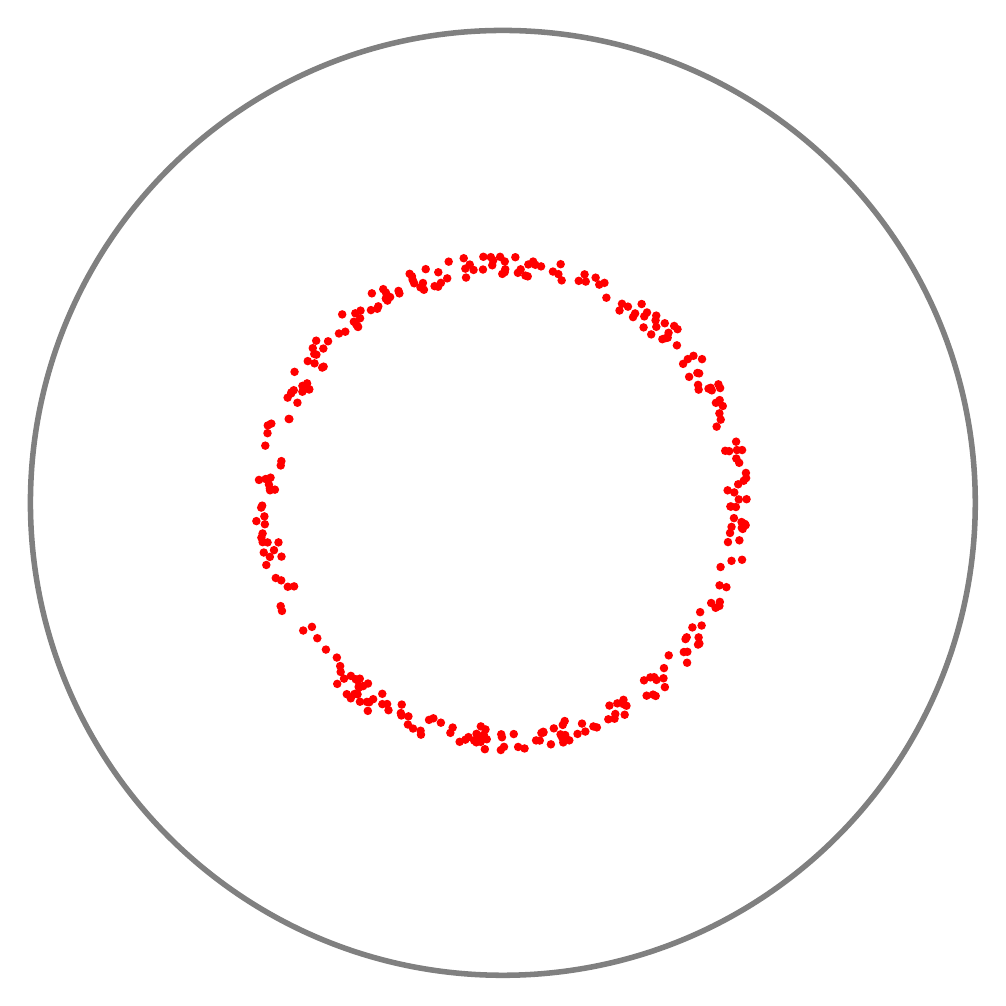
\begin{tikzpicture}[scale=0.06]
    \draw[line width=2pt, gray] (0,0) circle (100);
    \foreach \i in {1,...,320}{
      \pgfmathsetmacro{\ang}{rnd*360}
      \pgfmathsetmacro{\rad}{50 + 5*(rnd-0.5)}
      \fill[red] (\ang:\rad) circle (0.9);
    }
  \end{tikzpicture}%
}

% ---- 内蔵図: 6層中1層ボイド断面 ----
\newcommand{\figPZTLayersVoidInline}{%
  \begin{tikzpicture}[x=1cm,y=1cm]
    \def\W{6.0}\def\H{0.45}\def\G{0.10}
    \foreach \i in {0,...,5}{
      \pgfmathsetmacro{\y}{\i*(\H+\G)}
      \draw[fill=gray!20] (0,\y) rectangle (\W,\y+\H);
    }
    % 4層目ボイド(矩形)
    \pgfmathsetmacro{\yv}{3*(\H+\G)}
    \draw[very thick,red] (2.2,\yv+0.10) rectangle (3.0,\yv+\H-0.10);
    % 上下に細線(電極/基板のイメージ)
    \draw[line width=1pt] (0,-0.30) -- (\W,-0.30);
    \draw[line width=1pt] (0,6*(\H+\G)+0.10) -- (\W,6*(\H+\G)+0.10);
  \end{tikzpicture}%
}

% ---- 内蔵図: 端部焼損模式(カラー)----
\newcommand{\figEdgeBurnoutInline}{%
  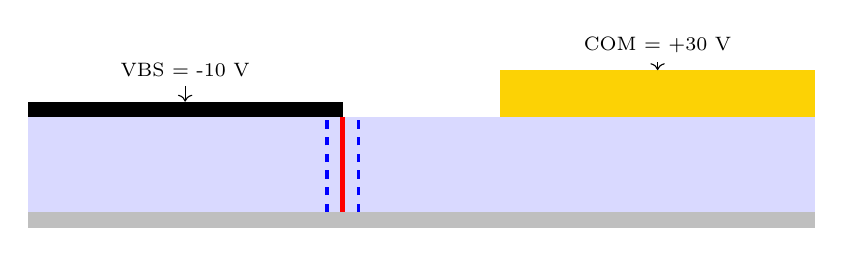
\begin{tikzpicture}[x=1cm,y=1cm]
    \def\W{10}\def\pztH{1.2}\def\beH{0.2}\def\teH{0.20}
    % Bottom Electrode
    \fill[gray!50] (0,0) rectangle (\W,\beH);
    % PZT
    \fill[blue!15] (0,\beH) rectangle (\W,\beH+\pztH);
    % Top Electrode (VBS)
    \fill[black] (0,\beH+\pztH) rectangle (4,\beH+\pztH+\teH);
    % Au Pad (COM)
    \fill[yellow!70!orange] (6,\beH+\pztH) rectangle (\W,\beH+\pztH+0.6);
    % Exposed sidewall
    \draw[line width=1.8pt,red] (4,\beH) -- (4,\beH+\pztH);
    % Proposed AlOx
    \draw[line width=1.2pt,blue,dashed] (3.8,\beH) -- (3.8,\beH+\pztH);
    \draw[line width=1.2pt,blue,dashed] (4.2,\beH) -- (4.2,\beH+\pztH);
    % Voltage labels(英数字のみ)
    \draw[->] (2, \beH+\pztH+\teH+0.2) -- (2,\beH+\pztH+\teH);
    \node[anchor=south] at (2, \beH+\pztH+\teH+0.2) {\scriptsize VBS = -10 V};
    \draw[->] (8, \beH+\pztH+0.7) -- (8,\beH+\pztH+0.6);
    \node[anchor=south] at (8, \beH+\pztH+0.7) {\scriptsize COM = +30 V};
  \end{tikzpicture}%
}

% ---- タイトル情報 ----
\title{PZT薄膜アクチュエータにおける振動板クラックと端部焼損の原因解析・対策提案}
\author{三溝 真一(Shinichi Samizo)\\
Independent Semiconductor Researcher\\
Former Engineer at Seiko Epson Corporation\\
\href{mailto:shin3t72@gmail.com}{shin3t72@gmail.com}\quad
GitHub: \url{https://github.com/Samizo-AITL}}
\date{}

\begin{document}
\maketitle

\begin{abstract}
Epson $\mu$TFP(薄膜PZT $d_{33}$)アクチュエータにおける
(1) 振動板クラック、(2) 端部焼損
の原因と対策を整理した。クラックはRTA後の疎水化によるスピン塗布時の気泡巻き込み(膜内ボイド)に起因し、
酢酸プレウェットで不良率を5--10\%からほぼ0\%に低減した。焼損は端部の側壁露出+40\,V差での電界集中が主因と推定し、
ALD-AlO$_x$被覆を対策案として提示する。
\end{abstract}

\section{序論}
Mach(バルク積層PZT, $d_{31}$, 180\,dpi)から、薄膜PZT TFP/$\mu$TFP($d_{33}$, 300\,dpi)へ移行し高密度化を達成したが、
薄膜特有の欠陥感受性と高電界により、クラック・焼損が顕在化した。

\section{デバイス・プロセス構成}
PZTはゾルゲル法で200\,nm$\times$6(総\SI{1.2}{\micro\meter})。
第1層焼成後にTi\SI{4}{\nano\meter}挿入。下電極Pt(111)/Ir seed、上電極Ir/Ti。
ドライバICは0.35\,\si{\micro m} CMOS, 3.3\,V/45\,V, 400ch$\times$2列。

\section{結果}
\subsection{クラック:同心リング分布と層内ボイド}
長期放置後の塗布・焼成で、反射条件最適化の検査により半径中間域にドーナツ状分布が観測された(図\ref{fig:donut})。
断面では6層中の特定層にボイドが局在(図\ref{fig:layer-void})。

\begin{figure}[H]\centering
  \figVoidDonutInline
  \caption{ウエハ上のドーナツ状ボイド分布(反射条件最適化)}
  \label{fig:donut}
\end{figure}

\begin{figure}[H]\centering
  \figPZTLayersVoidInline
  \caption{PZT 6層のうち1層にボイドを含む断面模式図}
  \label{fig:layer-void}
\end{figure}

\subsection{端部焼損:電界集中部位}
COM(Au配線)とVBS(上電極)が最接近する側壁露出部で焼損が発生。差分40\,Vの台形波立上りで瞬間電流が重畳し、局所絶縁破壊が誘発(図\ref{fig:edge})。

\begin{figure}[H]\centering
  \figEdgeBurnoutInline
  \caption{端部焼損の模式図(電界集中部とAlO$_x$対策案)}
  \label{fig:edge}
\end{figure}

\section{結論}
(1) クラックは「RTA後疎水化 $\rightarrow$ 気泡巻き込み $\rightarrow$ 膜内ボイド」の連鎖が原因で、酢酸プレウェット導入により不良率をほぼ0\%へ。
(2) 焼損は「側壁露出+電界集中」が主因と推定し、ALD-AlO$_x$被覆を提案。高密度・高電圧駆動化での量産信頼性設計に資する。

\section*{著者略歴}
\textbf{三溝 真一(Shinichi Samizo)} 信州大学大学院 電子情報工学専攻 修士。
セイコーエプソンにて半導体メモリ/ミックスドシグナル、薄膜PZT MEMSアクチュエータおよびPrecisionCoreプリントヘッド技術に従事。
現在は独立系半導体リサーチャとして、プロセス/デバイス教育、メモリアーキテクチャ、AI統合制御に注力。
\textbf{Contact:} \href{mailto:shin3t72@gmail.com}{shin3t72@gmail.com}。

\end{document}
